
\section{Theoretical Minimum}

\subsection{Nature of classical physics}

\begin{answer}
	Closed systems can actually exist if the collection of objects under investigation do not interact with anything outside of the system.

	Consider the empty system $\emptyset$, an empty collection that contains no objects.
	The empty system is a closed system that actually exists.

	Implicit in establishing a closed system are the assumptions that all interactions with its objects are known and can be definitively measured.
	An open system is a system that interacts with objects outside the system.

	As a matter of logic, a system should be presumed closed and shown to be open.
	However, the failure to establish a system to be open does not suffice to definitively conclude the system is closed.
\end{answer}

% functions of states 
\begin{answer}
	Consider a system consisting of six states $S = \left\{1, 2, 3, 4, 5, 6\right\}$.

	A law is given by a function $S \xrightarrow{f} S$ that assigns each state in $S$ to the state that results from evolution under the law.

	If any law is allowed, then the set of laws is given by the set of all functions from $S$ to $S$.

	If a law must satisfy the conservation of information, then the set of laws that are possible for a six-state system can be classified by the set of functions
	\begin{align}
		C & = \left\{ f : S \to S \mid \forall y \in S, \exists!\ x \in S. f(x) = y \right\},
	\end{align}
	where each function has the property that each element in its codomain has a corresponding, unique element in the domain that is mapped to it and thus each such function in $C$ is a bijection.
	The number of such laws, given by the size $\left|C\right| = 6!$ of $C$, is $6 \times 5 \times 4 \times 3 \times 2 \times 1 = 720$.
	This is because any function $S \xrightarrow{f} S$ in $C$ can be defined by sampling from the space $S$ of outcomes six times without replacement.
\end{answer}

\begin{answer}
	Consider the infinite system $\left\{\cdots, -1, 0, +1, +2, \cdots\right\}$.

	Examples of dynamical laws that are allowable include those given by the following equations.
	\begin{align}
		N(n+1) = N(n) - 1 \quad
		N(n+1) = N(n) + 2 \quad
		N(n+1) = -1^{N(n)} N(n)
	\end{align}
	On the other hand, the dynamical law given by the equation $N(n+1) = N(n)^2$ is not allowed because it does not satisfy the conservation of information.
\end{answer}

\subsubsection{Spaces, srigonometry, and vectors}
\setcounter{answer}{0}

\begin{answer}
	Consider the functions $f,g,\theta,t$ defined below.
	\begin{align}
		f(t)           & = t^4 + 3t^3 - 12t^2 + t - 6   \\
		g(x)           & = \sin x - \cos x              \\
		\theta(\alpha) & = e^\alpha + \alpha \ln \alpha \\
		t(x)           & = \sin^2x - \cos x
	\end{align}

	They are plotted in Figure \ref{fig:plot} above.
	\begin{figure}
		
% sciences/science/assets/plot.tex

\begin{subfigure}{0.32\textwidth}\centering
	\begin{tikzpicture}
		\begin{axis}[width=1\linewidth, legend pos=north east, legend style={font=\tiny}]
			\addplot[variable=t]{t^4 + 3*t^3 - 12*t^2 + t - 6  };
			\addlegendentry{$f(t) = t^4 + 3t^3 - 12t^2 + t - 6$}
		\end{axis}
	\end{tikzpicture}
	\caption{Plot of $f(t)$}
\end{subfigure}
\hfill
\begin{subfigure}{0.32\textwidth}\centering
	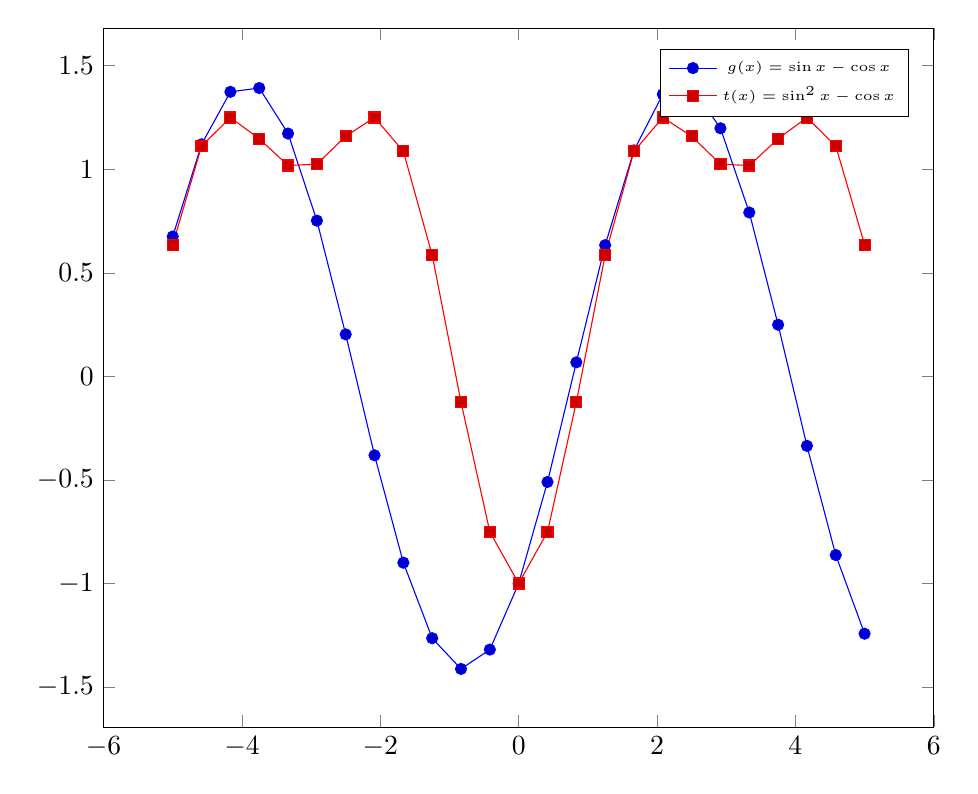
\begin{tikzpicture}
		\begin{axis}[trig format=rad, width=1\linewidth, legend pos=north east, legend style={font=\tiny}]
			\addplot{sin(x) - cos(x)};
			\addlegendentry{$g(x) = \sin x - \cos x$}
			\addplot{sin(x)^2 - cos(x)};
			\addlegendentry{$t(x) = \sin^2 x - \cos x$}
		\end{axis}
	\end{tikzpicture}
	\caption{Plot of $g(x)$ and $t(x)$}
\end{subfigure}
\hfill
\begin{subfigure}{0.32\textwidth}\centering
	\begin{tikzpicture}
		\begin{axis}[width=1\linewidth, legend pos=north east, legend style={font=\tiny}]
			\addplot[variable=\alpha]{e^(\alpha) + \alpha * ln(\alpha)};
			\addlegendentry{$\theta(\alpha) = e^\alpha + \alpha \ln \alpha$}
		\end{axis}
	\end{tikzpicture}
	\caption{Plot of $\theta(\alpha)$}
\end{subfigure}


		\caption{Plots of functions}
		\label{fig:plot}
	\end{figure}
\end{answer}

\begin{answer}
	The rule for vector subtraction is to add the augend add the result of reversing the direction of the addend.

	Any vectors $\vec{A}$ and $\vec{B}$ satisfy the following equation.
	\begin{align}
		\vec{A} - \vec{B} & = \vec{A} + \left(-\vec{B}\right)
	\end{align}
\end{answer}

\begin{answer}
	For any vector $\vec{A}$, the magnitude $\left| \vec{A} \right| = \sqrt{A_x^2 + A_y^2 + A_z^2}$ of $\vec{A}$ satisfies the following equations:
	\begin{align}
		\vec{A} \cdot \vec{A} & = A_x A_x + A_y A_y + A_z A_z & = \left| \vec{A} \right|^2.
	\end{align}
\end{answer}

\begin{answer}
	Let $\left(A_x = 2, A_y = -3, A_z = 1\right)$ and $\left(B_x=-4, B_y=-3, B_z=2\right)$.

	The magnitude $\left|\vec{A}\right| = \sqrt{2^2 + (-3)^2 + 1^2}$ of $\vec{A}$ is $\left|\vec{A}\right| = \sqrt{4+9+1} = \sqrt{14}$, and the magnitude $\left|\vec{B}\right| = \sqrt{(-4)^2 + (-3)^2 + 2^2}$ of $\vec{B}$ is $\left|\vec{B}\right| = \sqrt{29}$.
	The dot product $\vec{A} \cdot \vec{B} = 2(-4) + (-3)(-3) + 1(2)$ of $\vec{A}$ and $\vec{B}$ is $\vec{A} \cdot \vec{B} = 3$.
	Since the angle $\theta$ between the two vectors satisfies $\vec{A} \cdot \vec{B} = \left|\vec{A}\right| \left|\vec{B}\right| \cos \theta$, it is given by $\dsp \theta = \cos^{-1} \frac{3}{\sqrt{406}}$ and approximated by $1.421$ radians.
\end{answer}

\begin{answer}
	Consider the vectors $(1,1,1)$, $(2,-1,3)$, $(3,1,0)$, and $(-3,0,2)$.
	The only pair of orthogonal vectors is $\left\{(2,-1,3), (-3,0,2)\right\}$.
\end{answer}

\begin{answer}
	The angle $\theta$ between two vectors that are orthogonal is $\frac{\pi}{2}$ radians, so their dot product is $\cos \frac{\pi}{2} = 0$.
\end{answer}

\subsection{Motion}

\begin{answer}
	Consider the functions $f,g,\theta,t$ defined by $f(t) = t^4 + 3t^3 - 12t^2 + t - 6$, $g(x) = \sin x - \cos x$, $\theta(\alpha) = e^\alpha + \alpha \ln \alpha$, and $t(x) = \sin^2x - \cos x$.

	The derivatives are given below.
	\begin{align*}
		\frac{df}{dt}           & = 4t^3 + 9t^2 - 24t + 1                \\
		\frac{dg}{dx}           & = \cos x + \sin x                      \\
		\frac{d\theta}{d\alpha} & = e^\alpha + 1 + \ln \alpha            \\
		\frac{dt}{dx}           & = \left(2 \sin x\right)\cos x + \sin x
	\end{align*}
\end{answer}

\begin{answer}
	Consider the functions $f,g,\theta,t$ defined by $f(t) = t^4 + 3t^3 - 12t^2 + t - 6$, $g(x) = \sin x - \cos x$, $\theta(\alpha) = e^\alpha + \alpha \ln \alpha$, and $t(x) = \sin^2x - \cos x$.

	The second derivatives are given below.
	\begin{align*}
		\frac{d^2f(t)}{dt^2}                & = 12t^2 + 18t - 24                                                   \\
		\frac{d^2g(x)}{dx^2}                & = \cos x - \sin x                                                    \\
		\frac{d^2\theta(\alpha)}{d\alpha^2} & = e^\alpha + \frac{1}{\alpha}                                        \\
		\frac{d^2t(x)}{dx^2}                & = -\left(2\sin x\right)\sin x + \left(2 \cos x\right)\cos x + \cos x
	\end{align*}
\end{answer}

\begin{answer}
	Consider the functions $g,\theta,x$ defined by $g(t) = \sin t^2 - \cos t^2$, $\theta(\alpha) = e^{3 \alpha} + 3 \alpha \ln 3 \alpha$, and $x(t) = \sin^2 t^2 - \cos t^2$.

	The chain rule yields $\frac{dg}{dt} = 2t \cos t^2 + 2t \sin t^2\dots$, $\frac{d\theta}{d\alpha} = 3e^{3\alpha} + 1 + 3\ln 3\alpha$, and $\frac{dx}{dt} = 4t\sin t^2 + 2t \sin t^2$.
\end{answer}

\begin{answer}
	The sum rule is shown for any $f$ and $g$ below.
	\begin{align*}
		\frac{d(f+g)}{dt} & =
		\lim_{\Delta t \to 0} \frac{\left(f(t+\Delta t)+g(t+\Delta t)\right)-\left(f(t)+g(t)\right)}{\Delta t}                                      \\
		                  & = \lim_{\Delta t \to 0} \frac{\left(f(t+\Delta t)-f(t)\right)+\left(g(t+\Delta t)-g(t)\right)}{\Delta t}                \\
		                  & = \lim_{\Delta t \to 0} \frac{f(t+\Delta t)-f(t)}{\Delta t} + \lim_{\Delta t \to 0} \frac{g(t+\Delta t)-g(t)}{\Delta t} \\
		                  & = \frac{df}{dt} + \frac{dg}{dt}
	\end{align*}
	The product rule for any $f$ and $g$ is shown below.
	\begin{align*}
		f(t)\frac{d(g)}{dt} + g(t) \frac{d(f)}{dt}
		 & = \lim_{\Delta t \to 0} f(t) \cdot \lim_{\Delta t \to 0} \frac{g(t+\Delta t)-g(t)}{\Delta t} + \lim_{\Delta t \to 0} g(t+\Delta t) \cdot \lim_{\Delta t \to 0} \frac{f(t+\Delta t) - f(t)}{\Delta t} \\
		 & = \lim_{\Delta t \to 0} \frac{f(t)g(t+\Delta t) - f(t)g(t) + g(t+\Delta t)f(t+\Delta t) - g(t+\Delta t)f(t)}{\Delta t}                                                                               \\
		 & = \lim_{\Delta t \to 0} \frac{f(t+\Delta t)g(t+\Delta t) - f(t)g(t)}{\Delta t}
		\frac{d\left(fg\right)}{dt}
	\end{align*}
	The chain rule for any $f$ and $g$ is shown below.
	\begin{align*}
		\frac{d\left(f(g(t))\right)}{dg(t)} \frac{d\left(g(t)\right)}{dt} & = \lim_{\Delta t \to 0} \frac{f\left(g(t)+(g(t+\Delta t) - g(t)) \right)-f\left(g(t)\right)}{g(t+\Delta t)-g(t)} \lim_{\Delta t \to 0} \frac{g(t+\Delta t) - g(t)}{\Delta t} \\
		                                                                  & = \lim_{\Delta t \to 0} \frac{f\left(g(t+\Delta t)\right) - f\left(g(t)\right)}{\Delta t}                                                                                    \\
		                                                                  & = \frac{d\left(f(g(t))\right)}{dt}
	\end{align*}
\end{answer}

\begin{answer}
	Recall the angle addition formula given below.
	\begin{align}
		\sin\left(\alpha + \beta\right) & = \sin \alpha \cos \beta + \cos \alpha \sin \beta \\
		\cos\left(\alpha + \beta\right) & = \cos \alpha \cos \beta - \sin \alpha \sin \beta \\
		% \tan\left(\alpha - \beta\right) & = \frac{\tan \alpha - \tan \beta}{1 + \tan \alpha \tan \beta} \label{eqn:tan}
	\end{align}
	Let $D = \left[-\frac{\pi}{2}, +\frac{\pi}{2}\right] \setminus \left\{0\right\}$.

	Recall that any $\theta \in D$ satisfies $\dsp \sin \theta < \theta < \tan \theta$.

	Division by $\theta$ yields $\dsp \frac{\sin \theta}{\theta} < 1 < \frac{\tan \theta}{\theta}$ and multiplication by $\cos \theta$ yields $\cos \theta < \frac{\sin \theta}{\theta}$.
	The squeeze theorem yields $\dsp \lim_{\theta \to 0} \cos \theta \leq \lim_{\theta \to 0} \frac{\sin \theta}{\theta} \leq \lim_{\theta \to 0} 1$ and thus $\dsp \lim_{\theta \to 0} \frac{\sin \theta}{\theta} = 1$.

	Observe $\dsp \frac{d\left(\sin t\right)}{dt} = \lim_{\Delta t \to 0} \frac{\left(\sin t \cos \Delta t + \cos t \sin \Delta t\right) - \sin(t)}{\Delta t} = 0 + 1 \cos t$ and
	$\dsp \frac{d\left(\cos t\right)}{dt} = \lim_{\Delta t \to 0} \frac{\left(\cos t \cos \Delta t - \sin t \sin \Delta t\right) - \cos t}{\Delta t} = 0 - 1 \sin t$.

	It follows from the definition of $e^t$ that $\dsp \frac{d\left(e^t\right)}{dt} = e^t$.

	If $x = \ln t$ for $t>0$, then the derivative of $t = e^x$ satisfies the equations $\dsp 1 = \frac{dt}{dt} = \frac{d\left(e^{x(t)}\right)}{dt} = e^x \frac{dx}{dt}$ and $\dsp \frac{d\left(\ln t\right)}{dt} = \frac{dx}{dt} = \frac{1}{e^x} = \frac{1}{t}$.
\end{answer}

\begin{answer}
	If the position of the particle is governed by $x(t) = \sin \omega t$, then the amount of time it takes for the oscillating particle to go through one full cycle of motion is $\dsp \frac{2 \pi}{\omega}$.
\end{answer}

\begin{answer}
	The dot product of the position and velocity vectors is given below.
	\begin{align}
		\begin{bmatrix}
			R \cos \omega t \\
			R \sin \omega t
		\end{bmatrix}
		\cdot
		\begin{bmatrix}
			-R \omega \sin \omega t \\
			R \omega \cos \omega t
		\end{bmatrix}
		= (R \sin \omega t)(R \omega \cos \omega t) - (R \cos \omega t)(R \omega \sin \omega t)
	\end{align}
	Since their dot product is $0$, the vectors are orthogonal.
\end{answer}

\begin{answer}
	The position vector $\dsp \vec{r} = \left(\cos \omega t, e^{\omega t}\right)$ has velocity $\left(\omega \sin \omega t, \omega e^{\omega t}\right)$, acceleration $\left(-\omega^2 \cos \omega t, \omega^2 e^{\omega t}\right)$, and speed $\omega \sqrt{\sin^2 \omega t + e^{2 \omega t}}$.
	The position vector $\dsp \vec{r} = \left(\cos(\omega t - \phi), \sin(\omega t - \phi)\right)$ has velocity $\dsp \left(\omega \sin(\omega t - \phi), -\omega \cos(\omega t - \phi)\right)$, acceleration $\dsp \left(-\omega^2 \cos(\omega t-\phi), -\omega^2\sin(\omega t-\phi)\right)$, and speed $\omega^2$.
	The position vector $\dsp \left(c \cos^3 t, c \sin^3 t\right)$ has velocity $\dsp \left(-3c (\sin t)\cos^2 t, 3c(\cos t)\sin^2 t\right)$, acceleration $\dsp \left(6c (\cos t)\sin^2 t - 3c\cos^3 t, 6c (\sin t)\cos^2 t - 3c\sin^3 t\right)$, and speed $9c^2(\sin^2 t)(\cos^2 t)$.
	The position vector $\dsp \vec{r} = \left(c(t-\sin t), c(1-\cos t)\right)$ has velocity $\dsp \left(c - c\cos t, c + c\sin t\right)$, acceleration $\dsp \left(c\sin t, - c\cos t\right)$, and speed $\dsp 2c^2\left(1 - \cos t + 2c^2\sin t\right) + 1$.
\end{answer}

\subsubsection{Calculus}
\setcounter{answer}{0}

\begin{answer}
	Consider the functions $f_1, f_2, f_3$ defined below.
	\begin{align}
		f_1(t) & = t^4     \\
		f_2(t) & = \cos t  \\
		f_3(t) & = t^2 - 2
	\end{align}
	The indefinite integrals are $\dsp \int t^4 ~dt = \frac{t^5}{5} + c$, $\dsp \int \cos t ~dt = \sin t + c$, and finally $\dsp \int t^2-2 ~dt = \frac{t^3}{3} - 2t + c$.
\end{answer}

\begin{answer}
	The fundamental theorem of calculus yields $\dsp \int_0^T t^4 ~dt = \frac{T^5}{5} - \frac{0^5}{5}$, $\dsp \int_0^T \cos t = \sin T - 0$, and $\dsp \int_0^T t^2-2 ~dt = \frac{T^3}{3} - 2T$.
\end{answer}

\begin{answer}
	The velocities $\dsp v_1(t) = \int_0^t {t'}^4~dt'$ has trajectory $\dsp \int_0^T \left(\frac{t^5}{5} - \frac{0}{5}\right) ~dt = \frac{T^6}{30} - 0$.
\end{answer}

\subsection{Dynamics}

\begin{answer}
	Consider a force that varies with time according to $F = 2t^2$ and with initial condition $x(0) = \pi$ at time $0$.
\end{answer}
